\documentclass{report}
\usepackage[spanish]{babel}
\usepackage[margin=2cm]{geometry}
\usepackage{graphicx}
\usepackage{float}
\usepackage{titlesec}
\usepackage{caption}
\usepackage{listings}
\usepackage{xcolor}
\usepackage{array}
\usepackage{booktabs}
\usepackage{tabularx}

\definecolor{codegreen}{rgb}{0,0.6,0}
\definecolor{codegray}{rgb}{0.5,0.5,0.5}
\definecolor{codepurple}{rgb}{0.58,0,0.82}
\definecolor{backcolor}{rgb}{0.95,0.95,0.95}


\lstset{
    basicstyle=\ttfamily,
    inputencoding=utf8,
    extendedchars=true,
    literate=%
    {á}{{\'a}}1
    {é}{{\'e}}1
    {í}{{\'i}}1
    {ó}{{\'o}}1
    {ú}{{\'u}}1
    {ñ}{{\~n}}1
    {Á}{{\'A}}1
    {É}{{\'E}}1
    {Í}{{\'I}}1
    {Ó}{{\'O}}1
    {Ú}{{\'U}}1
    {Ñ}{{\~N}}1
}


\lstdefinestyle{mystyle}{
    backgroundcolor=\color{backcolor},
    commentstyle=\color{codegreen},
    keywordstyle=\color{red},
    numberstyle=\tiny\color{codegray},
    stringstyle=\color{codepurple},
    basicstyle=\ttfamily\footnotesize,
    breakatwhitespace=false,
    breaklines=true,
    captionpos=b,
    keepspaces=true,
    numbers=left,
    showspaces=false,
    showstringspaces=false,
    showtabs=false,
    tabsize=2  
}

\titleformat{\section}
{\huge\bfseries}{\thesection.}{1em}{}
\titleformat{\subsection}
{\large\bfseries}{\thesubsection}{1em}{}

\renewcommand\thesection{\arabic{section}}

\title{\Huge{\textbf{Practica 3. Algoritmo Evolutivos: Estrategias Evolutivas y Evolución Diferencial.}}\\
\Large{\textbf{Algoritmos Bioinspirados}}}
\author{Diego Castillo Reyes\\Marthon Leobardo Yañez Martinez\\Aldo Escamilla Resendiz}

\graphicspath{{imagenes/}}

\begin{document}
    \maketitle
    \tableofcontents
    \newpage
    \section{Introducción}
    Los Algoritmos Evolutivos son una familia de métodos de optimización inspirados en el proceso de selección natural y evolución biológica. Dos enfoques destacados dentro de esta familia son las **Estrategias Evolutivas** y la **Evolución Diferencial**, cada uno con sus particularidades y aplicaciones.
Estrategias Evolutivas (ES)

Las Estrategias Evolutivas son técnicas que se centran principalmente en la optimización numérica continua. En estas estrategias, la población de soluciones evoluciona a través de la mutación y la selección. La mutación se realiza generalmente mediante la adición de ruido normalmente distribuido a los vectores de parámetros, lo que permite una exploración efectiva del espacio de búsqueda. Una característica distintiva de las ES es el uso de mecanismos de autoadaptación para ajustar los parámetros de la mutación, como la tasa de mutación, basándose en el éxito de las generaciones anteriores.

Evolución Diferencial (DE)
La Evolución Diferencial es otro método robusto para optimizar problemas de optimización numérica. Se caracteriza por su sencillez y eficacia, especialmente en problemas multimodales (con múltiples óptimos locales). En DE, la nueva generación se crea añadiendo la diferencia ponderada entre dos o más soluciones de la población actual a una tercera solución. Este método se basa en operadores simples como la mutación diferencial, la recombinación y la selección. La mutación diferencial es particularmente útil para mantener la diversidad genética dentro de la población, lo que ayuda a explorar de manera efectiva el espacio de búsqueda.

Ambos métodos, aunque similares en su inspiración evolutiva, difieren en sus mecanismos de mutación y adaptación, lo que los hace adecuados para diferentes tipos de problemas de optimización. La elección entre Estrategias Evolutivas y Evolución Diferencial a menudo depende del problema específico, la naturaleza del espacio de búsqueda y las preferencias del investigador o ingeniero.

\section{Desarrollo}
Para el desarrollo de esta práctica se programaron los siguientes codigos.
\subsection{Estrategia Evolutiva ($\mu , \lambda$)}
Usa una estrategia evolutiva en la que solo los descendientes (no los padres) son considerados para la generación siguiente, lo que puede ayudar a evitar la convergencia prematura hacia mínimos locales subóptimos.
\lstinputlisting[language=Python, style=mystyle]{estrategiaEvolutiva1.py}
Este código es una implementación directa de una estrategia evolutiva que facilita la optimización en espacios de búsqueda complejos mediante la adaptación continua de los parámetros y el uso de operadores genéticos como la mutación y el crossover.
\subsection{Estrategia Evolutiva ($\mu + \lambda$)}
\lstinputlisting[language=Python, style=mystyle]{estrategiaEvolutiva2.py}

\subsection{Evolución Diferencial}
\lstinputlisting[language=Python, style=mystyle]{evolucionDiferencial.py}

¿Cuáles fueron las versiones de algoritmos que no convergieron a la solución optima?\\
En la función Griewank, todas las ejecuciones tienden a converger hacia soluciones con valores de fitness relativamente bajos. Esto sugiere que no existen evidencias claras que indiquen la falta de convergencia en alguna de las variantes del algoritmo evaluadas. Por tanto, aunque el rendimiento puede no ser óptimo, todos los enfoques del algoritmo parecen alcanzar un cierto nivel de estabilidad en sus resultados.\\
¿A qué versión de estretegia evolutiva le fue mejor?\\
En la función Rastrigin, todas las estrategias evolutivas exhiben un rendimiento parecido, convergiendo hacia soluciones con valores de fitness bajos. Sin embargo, se observa una excepción notable en la segunda ejecución utilizando la Evolución Diferencial con la estrategia (rand/1/exp), que logró alcanzar un fitness significativamente superior. Esto sugiere que esta configuración particular del algoritmo puede ser más efectiva bajo ciertas condiciones, destacándose del resto en términos de eficacia.\\
¿Qué versión de evolucion diferencial fue la mejor e indique por que cree que le fue mejor (en qué problemas).\\
En la función Rastrigin, las estrategias de Evolución Diferencial (DE) utilizando tanto (rand/1/bin) como (best/1/bin) mostraron un desempeño destacado, logrando en varias ejecuciones converger hacia soluciones con un fitness cercano a cero, que representa el óptimo para esta función. Esto indica que estas estrategias podrían ser especialmente efectivas para abordar problemas que presentan múltiples óptimos locales, como es el caso de Rastrigin, debido a su eficiente balance entre exploración y explotación del espacio de búsqueda.

Por otro lado, en la función Griewank, todas las estrategias evaluadas parecen converger hacia soluciones con fitness bajo, lo que no permite identificar diferencias significativas en el rendimiento entre las distintas variantes de evolución diferencial aplicadas. Sin embargo, la estrategia DE (best/1/exp) mostró un rendimiento ligeramente superior en algunas de las ejecuciones, sugiriendo que podría tener ciertas ventajas en determinadas configuraciones o escenarios de este problema.\\

Considerando todas las pruebas, cuál es el algoritmo que converge mas rápido (respecto a suvalor de media)\\
El algoritmo de Evolución Diferencial (DE) utilizando la estrategia (rand/1/bin) se destaca por su rapidez en la convergencia, especialmente cuando se aplica a la función Rastrigin. En múltiples ejecuciones, este algoritmo ha demostrado su capacidad para converger eficientemente hacia soluciones con un fitness cercano a cero, el cual es el valor óptimo para esta función. Esta eficacia en alcanzar rápidamente soluciones de alta calidad lo convierte en una opción atractiva para problemas de optimización complejos con múltiples óptimos locales.\\

\begin{table}[ht]
    \centering
    \caption{Comparación de Métodos Evolutivos}
    \label{tab:comparacion_metodos}
    \begin{tabularx}{\textwidth}{X|X|X}
    \toprule
    \textbf{Algoritmo Genético} & \textbf{Evolución Diferencial} & \textbf{Estrategias Evolutivas} \\
    \midrule
    Utiliza operadores de cruzamiento y mutación. & Se basa en la combinación de soluciones ponderadas. & Utiliza mutaciones con adaptación de parámetros. \\
    \addlinespace
    Operan sobre una representación binaria o simbólica. & Opera sobre una representación real. & Opera generalmente sobre representaciones reales. \\
    \addlinespace
    Selección basada en el rendimiento relativo. & Selección directa por torneos entre individuos y sus mutantes. & Uso de técnicas de selección como la $(\mu, \lambda)$ y $(\mu+\lambda)$. \\
    \addlinespace
    Aplicación amplia en problemas de optimización combinatoria. & Eficiente en problemas de optimización sobre espacios continuos. & Enfocado en la auto-adaptación de las estrategias de búsqueda. \\
    \bottomrule
    \end{tabularx}
\end{table}

\begin{table}[ht]
\centering
\caption{Comparación de estrategias en diferentes funciones}
\begin{tabular}{>{\raggedright}p{3cm}ccccccc}
\toprule
\textbf{Problema} & \textbf{(m, $\lambda$)} & \textbf{(m + $\lambda$)} & \textbf{(r/1/b)} & \textbf{(r/1/e)} & \textbf{(b/1/b)} & \textbf{(b/1/e)} \\
\midrule
Ackley & 3.985e-15 & 3.9856e-15 & 1.0302 & 0.5505 & 0.7049 & 0.388 \\
Griewank & -- & 5.1222e-08 & 0 & 8.3599e-12 & -- & 7.233e-08 \\
Rastrigin & 1.790e-12 & 40.709 & 4.07 & 31.20 & 11.286 & 29.971 \\
Rosenbrock & 2.059e-14 & 4.6960e-15 & 12.8 & 12.292 & -- & 25.863 \\
\bottomrule
\end{tabular}
\end{table}

\section{Resultados}
\subsection{Resultados de estrategias evolutivas}
%inserta imagen 
\begin{figure}[H]
    \centering
    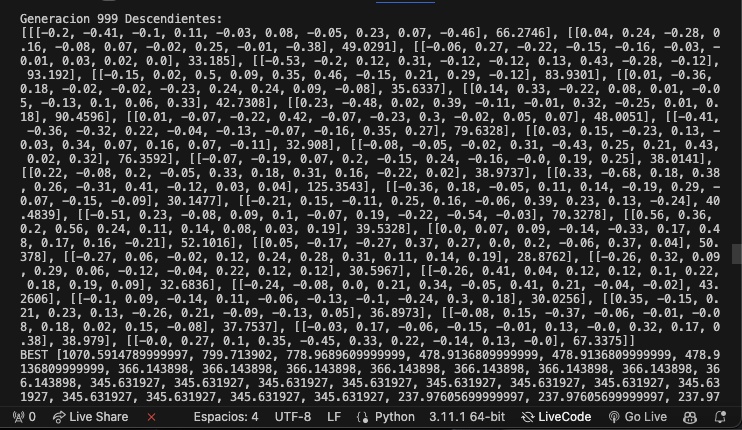
\includegraphics[width=1\textwidth]{evolutiva1.png}
    \caption{Resultados de estrategiaEvolutiva1}
\end{figure}
\begin{figure}[H]
    \centering
    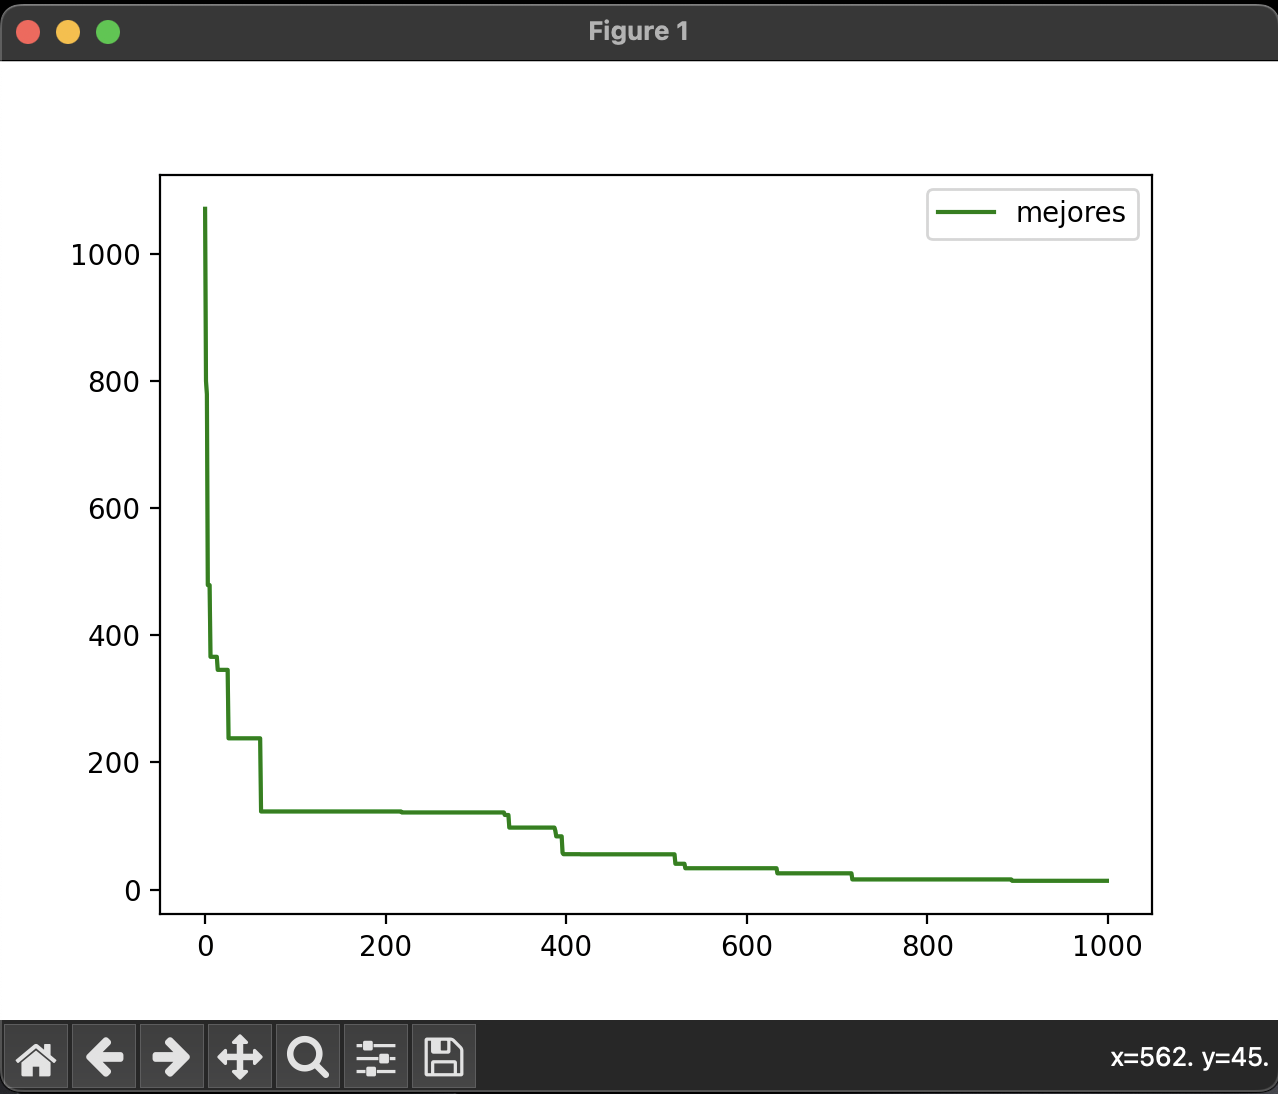
\includegraphics[width=1\textwidth]{graficaev1.png}
    \caption{Gráfica de resultados de estrategiaEvolutiva1}
\end{figure}

\begin{figure}[H]
    \centering
    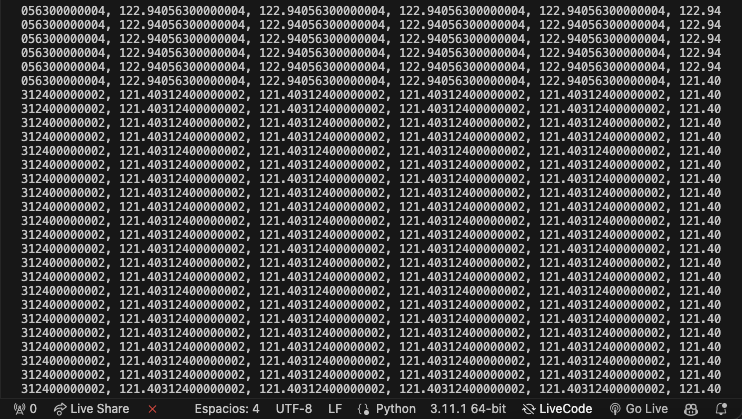
\includegraphics[width=1\textwidth]{evolutiva1.2.png}
    \caption{Resultados de estrategiaEvolutiva1}
\end{figure}

\begin{figure}[H]
    \centering
    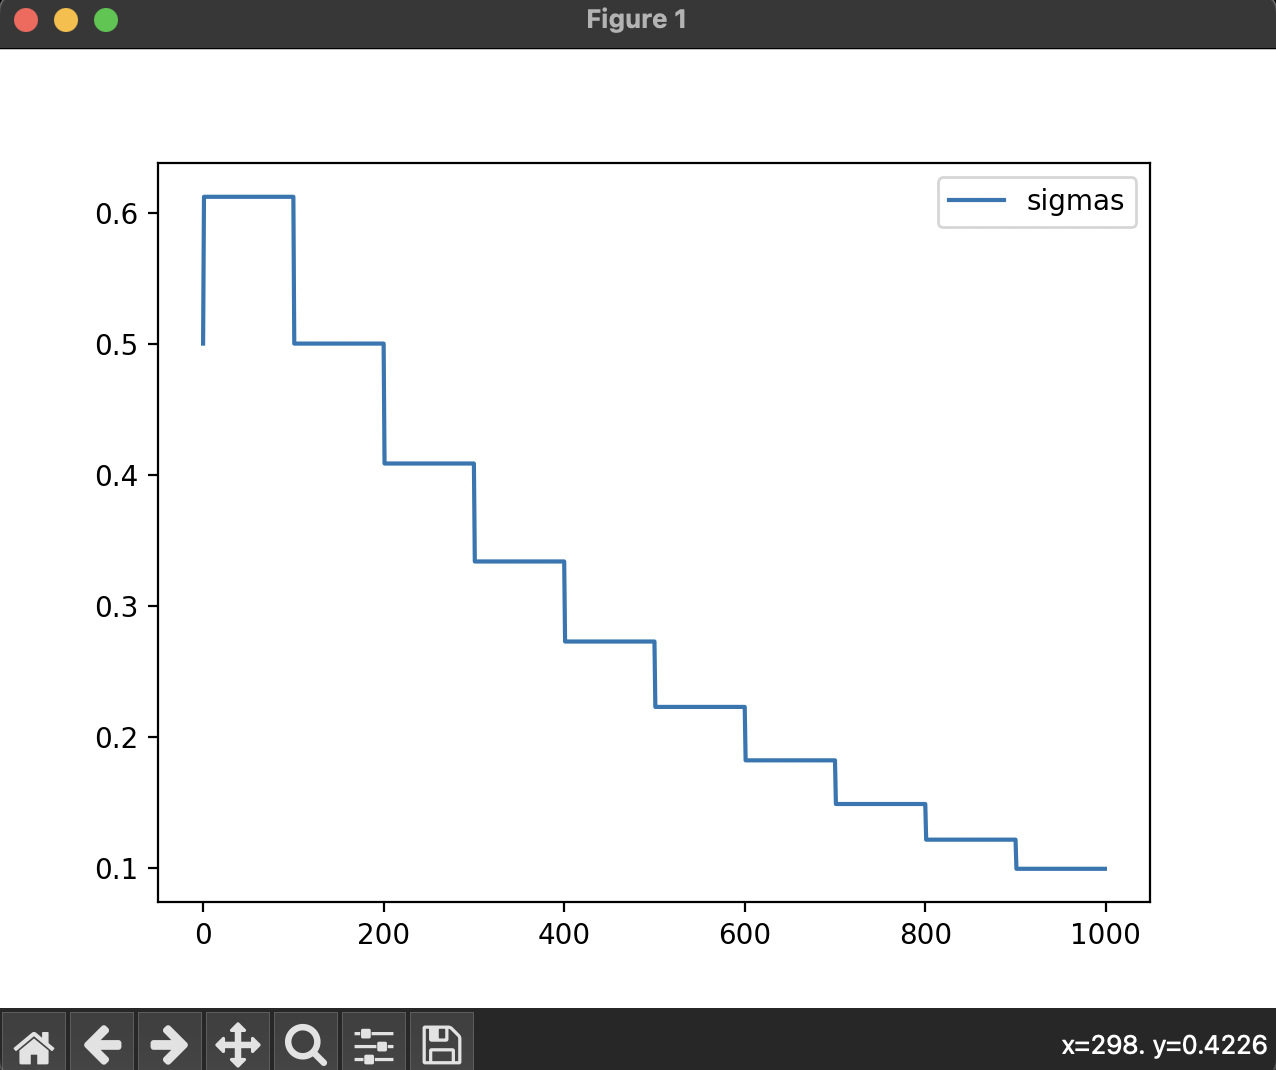
\includegraphics[width=1\textwidth]{graficaev1.2.png}
    \caption{Gráfica de resultados de estrategiaEvolutiva1}
\end{figure}

\begin{figure}[H]
    \centering
    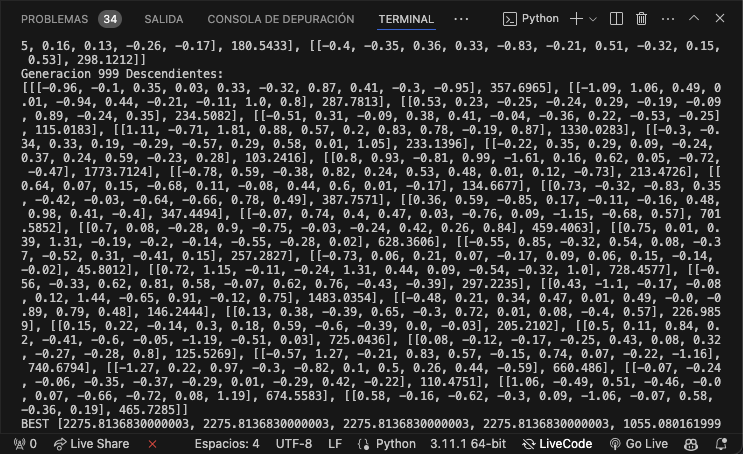
\includegraphics[width=1\textwidth]{evolutiva2.png}
    \caption{Resultados de estrategiaEvolutiva2}
\end{figure}

\begin{figure}[H]
    \centering
    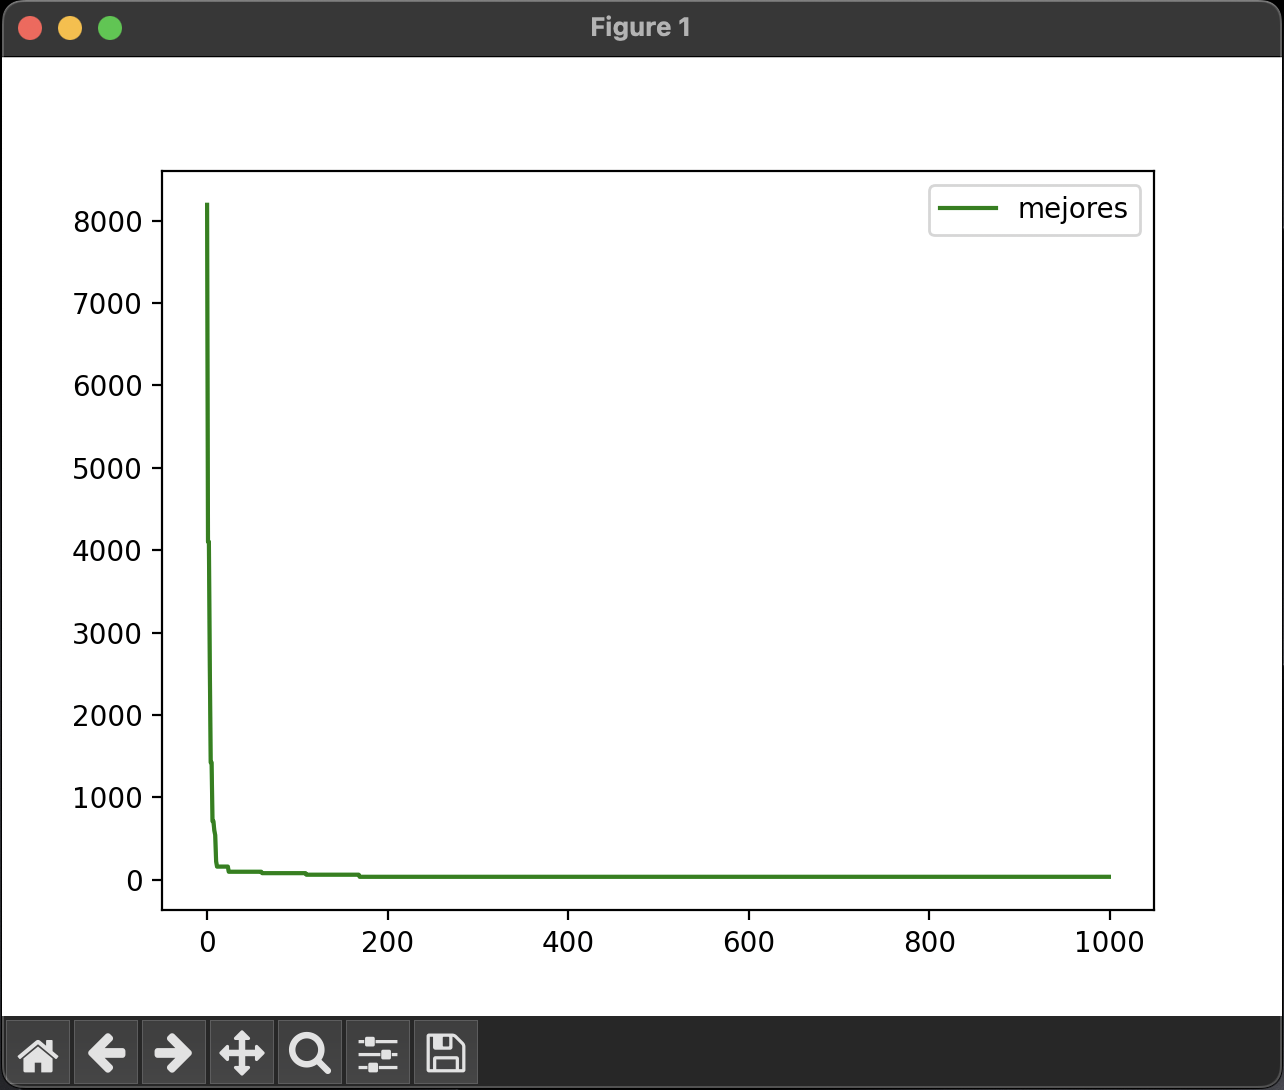
\includegraphics[width=1\textwidth]{graficaev2.png}
    \caption{Gráfica de resultados de estrategiaEvolutiva2}
\end{figure}

\subsection{Resultados de evolución diferencial}
\begin{figure}[H]
    \centering
    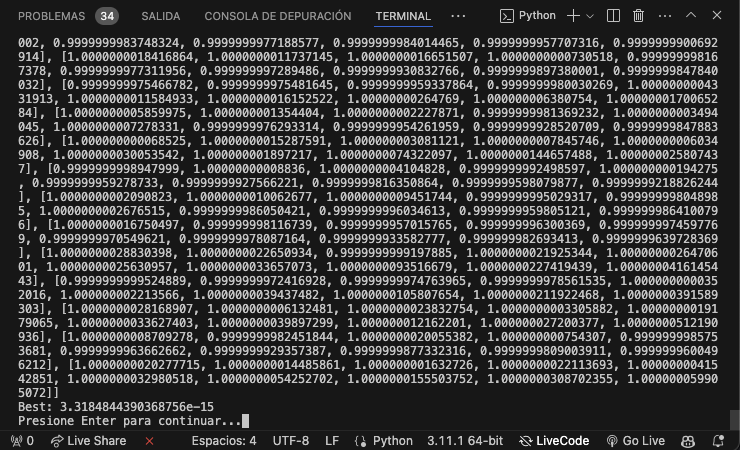
\includegraphics[width=1\textwidth]{evDif.png}
    \caption{Resultados de evolucionDiferencial.py}
\end{figure}

\begin{figure}[H]
    \centering
    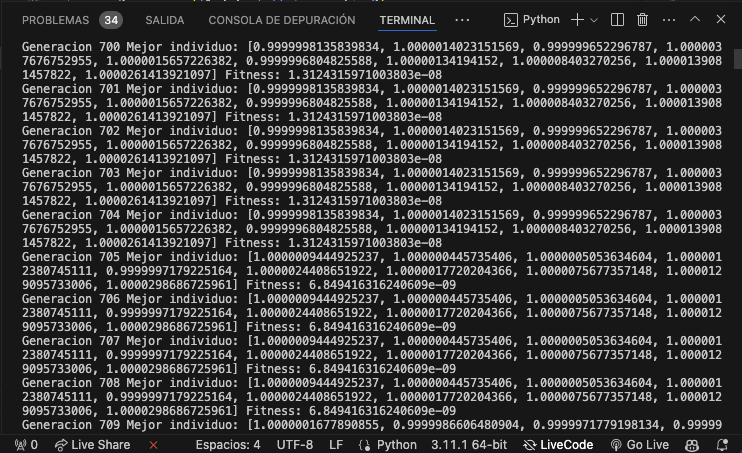
\includegraphics[width=1\textwidth]{generacionDif.png}
    \caption{Resultados generacionales de evolucionDiferencial.py}
\end{figure}

\section{Conclusiones}

Escamilla Resendiz Aldo\\
Los algoritmos de Evolución Diferencial (DE) han mostrado ser herramientas potentes y versátiles para abordar funciones de optimización complejas como Rastrigin y Griewank. Específicamente, la estrategia DE (rand/1/bin) se ha destacado por su rapidez en la convergencia hacia el óptimo en la función Rastrigin, mientras que las estrategias DE (rand/1/bin) y DE (best/1/bin) también han demostrado ser efectivas en enfrentar problemas con múltiples óptimos locales gracias a su capacidad para explorar y explotar eficientemente el espacio de búsqueda.\\
Castillo Reyes Diego\\
Todas las estrategias tendieron a converger a soluciones de baja fitness en la función Griewank, la DE (best/1/exp) ha mostrado un rendimiento ligeramente superior en ciertas ejecuciones. Esto sugiere que la elección de la estrategia DE puede ser crucial dependiendo de la naturaleza específica del problema de optimización a resolver.\\
Yañez Martinez Marthon\\
la importancia de elegir la estrategia adecuada de DE, adaptada a las características específicas del problema, para lograr un equilibrio óptimo entre exploración y explotación.

\end{document}
